\documentclass[border=10pt]{standalone}

\usepackage{tikz}
\usepackage{tikzsymbols}
\usetikzlibrary{calc,patterns,shapes.geometric}

\def\centerarc[#1](#2)(#3:#4:#5){\draw[#1] ($(#2)+({#5*cos(#3)},{#5*sin(#3)})$) arc (#3:#4:#5);}

\begin{document}
	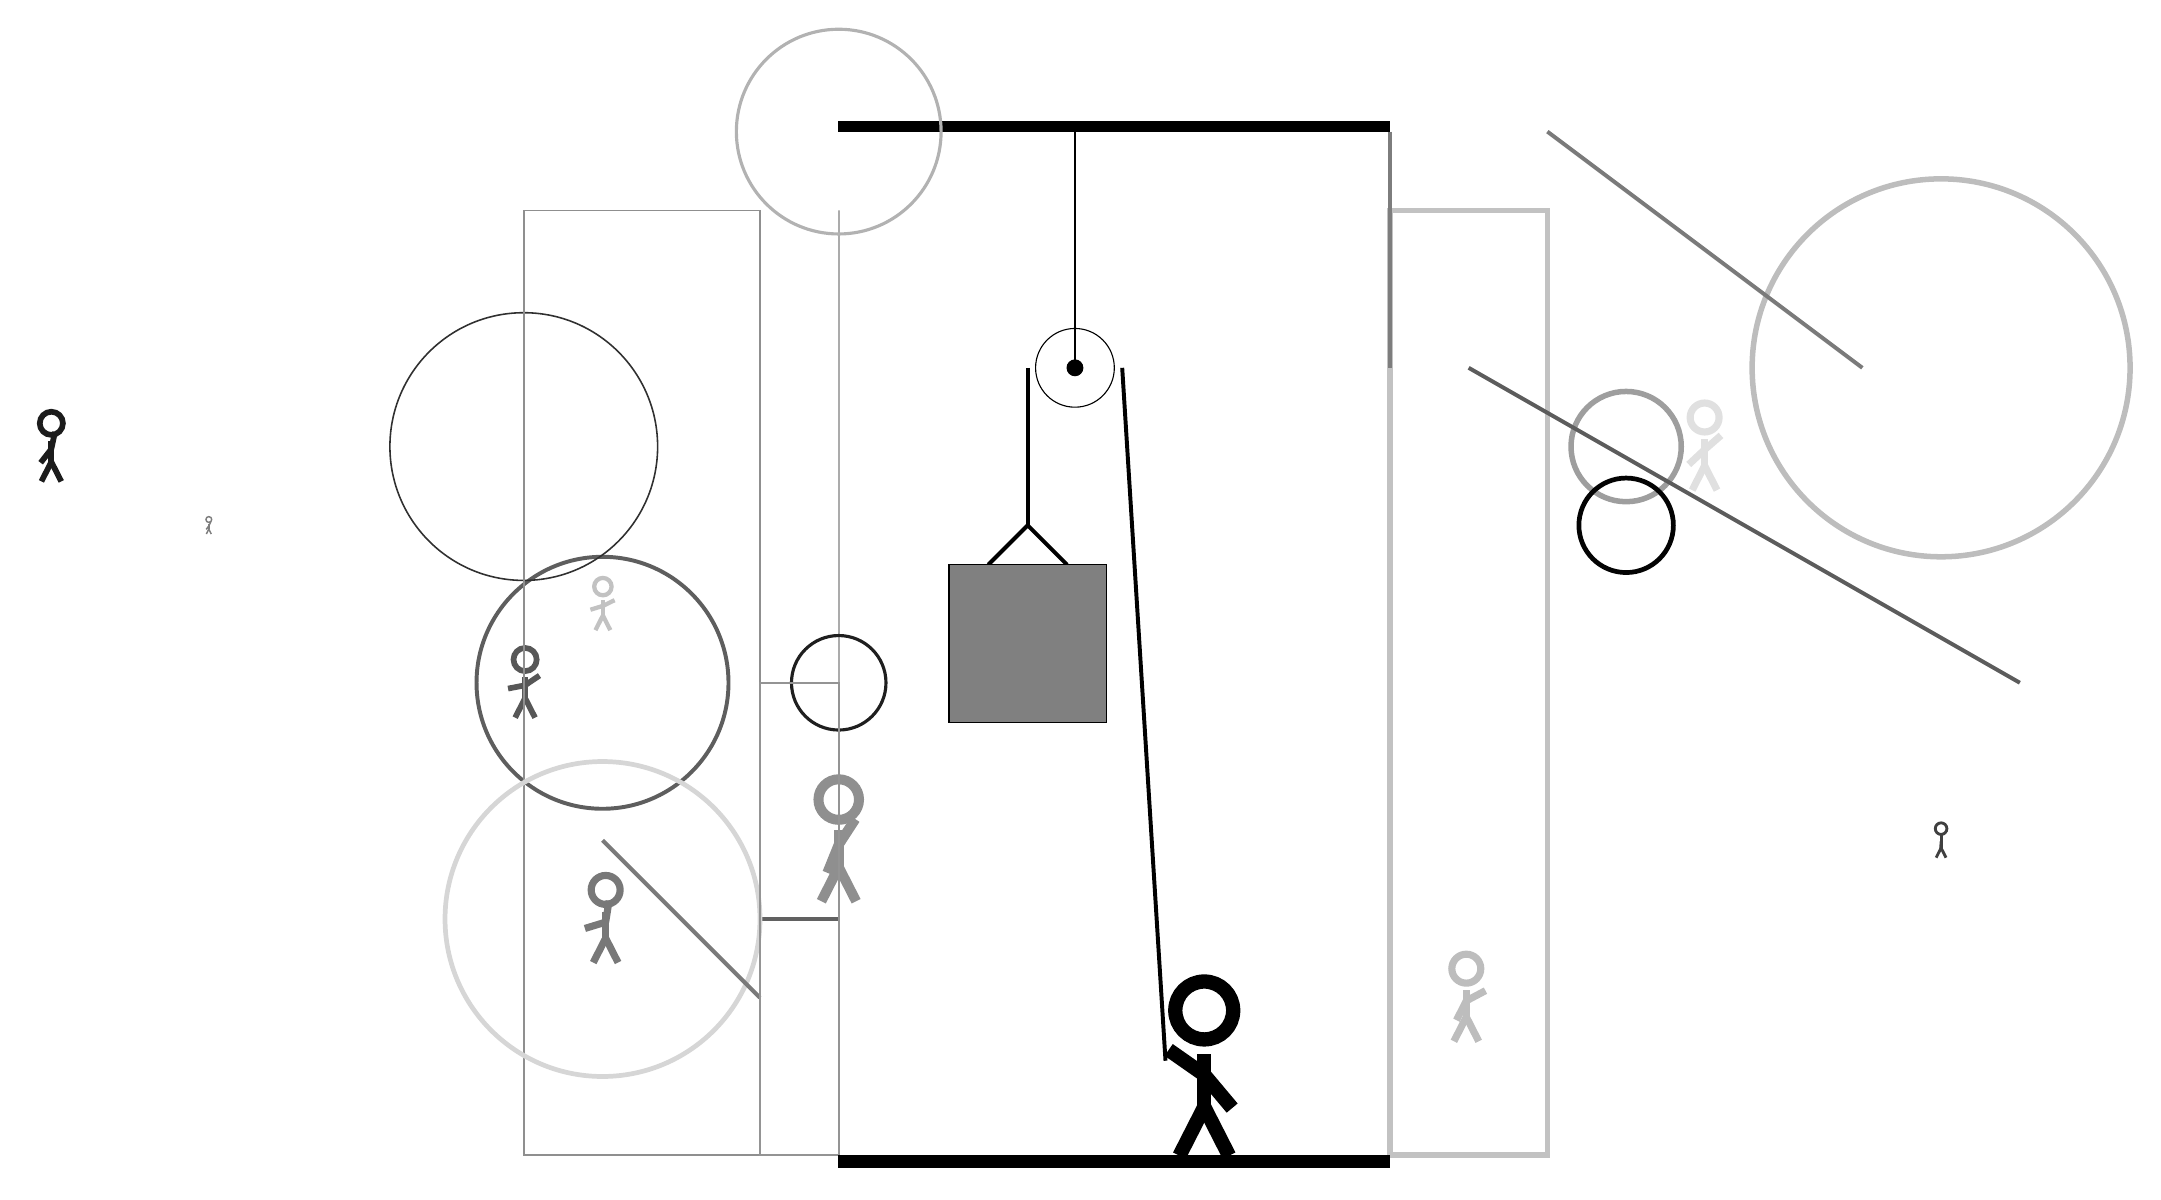
\begin{tikzpicture}
		%%%%% START %%%%%
		
		\draw[fill=black] (-2, 10) rectangle (5, 10.125);
		
		\draw (1, 7) circle (0.5);
		\draw[fill=black] (1, 7) circle (0.1);
		\draw (1, 10) -- (1, 7);
		
		\draw[line width=0.5mm] (-0.1, 4.5) -- (0.4, 5.0) -- (0.9, 4.5);
		\draw[fill=black!50] (-0.6, 4.5) rectangle (1.4, 2.5);
		
		\draw[line width=0.5mm] (0.4, 7) -- (0.4, 5.0);
		\centerarc[line width=0.5mm](1, 7)(0:180:0.6);
		\draw[line width=0.5mm](1.6, 7) -- (2.15, -1.8);
		
		\node[line width=0.4mm, color=black!89] at (-12, 6) {\Strichmaxerl[4][52][78]};
		
		\node[line width=0.5mm, color=black!53] at (-5, 0) {\Strichmaxerl[5][17][81]};
		\draw [line width=0.7mm, color=black!26](12, 7) circle (2.4);
		\node[line width=0.4mm, color=black!66] at (-6, 3) {\Strichmaxerl[4][11][34]};
		
		\draw[line width=0.6mm, color=black!62] (-2, 0) rectangle (-3, 0);
		\draw [line width=0.5mm, color=black!63](-5, 3) circle (1.6);
		
		\node[line width=0.2mm, color=black!44] at (-2, 1) {\Strichmaxerl[7][68][57]};
		
		\draw [line width=0.7mm, color=black!38](8, 6) circle (0.7);
		\draw[line width=0.7mm, color=black!24] (5, 9) rectangle (7, -3);
		\draw[line width=0.2mm, color=black!33] (-2, 9) rectangle (-2, -2);
		\draw [line width=0.4mm, color=black!88](-2, 3) circle (0.6);
		\node[line width=0.7mm, color=black!26] at (6, -1) {\Strichmaxerl[5][63][28]};
		\node[line width=0.6mm, color=black!51] at (-10, 5) {\Strichmaxerl[1][53][63]};
		
		\draw [line width=0.4mm, color=black!30](-2, 10) circle (1.3);
		\draw [line width=0.2mm, color=black!81](-6, 6) circle (1.7);
		\node[line width=0.7mm, color=black!75] at (12, 1) {\Strichmaxerl[2][87][90]};
		
		\draw[line width=0.5mm, color=black!52](7, 10) -- (11, 7);
		\draw[line width=0.2mm, color=black!44] (-3, -3) rectangle (-6, 9);
		\draw[line width=0.5mm, color=black!51](5, 10) -- (5, 7);
		\draw [line width=0.6mm, color=black!99](8, 5) circle (0.6);
		\draw [line width=0.6mm, color=black!16](-5, 0) circle (2.0);
		
		\draw[line width=0.5mm, color=black!52](-3, -1) -- (-5, 1);
		\draw[line width=0.3mm, color=black!42] (-3, 3) rectangle (-2, -3);
		\node[line width=0.6mm, color=black!24] at (-5, 4) {\Strichmaxerl[3][17][26]};
		\node[line width=0.2mm, color=black!12] at (9, 6) {\Strichmaxerl[5][43][41]};
		\draw[line width=0.5mm, color=black!64](6, 7) -- (13, 3);
		
		\node at (2.6, -1.9) {\Strichmaxerl[10][-35][-50]};
		
		\draw[fill=black] (-2, -3) rectangle (5, -3.15);
		
		%%%%% END %%%%%
	\end{tikzpicture}
\end{document}